\documentclass[12pt,a4paper]{article}
\usepackage[utf8]{inputenc} 
\usepackage[danish]{babel} 
\usepackage[T1]{fontenc} 
\usepackage{graphicx}
\usepackage{amsmath}
\usepackage[amsmath]{maxiplot}
\usepackage{tikz}

\def\Maxima{\emph{Maxima}}
\def\Gnuplot{\emph{Gnuplot}}

\begin{document}

\title{Eksempler på \Maxima{} og TikZ i \LaTeX{}.}
\author{Ole Guldberg, ole@omgwtf.dk}
\date{\today}
\maketitle

\section*{To linier}

De to linier $$-2x+7 = 2x-1$$ skæres i: 
$$\begin{maxima}
  tex(solve(-2*x+7=2*x-1,x))
\end{maxima}
$$
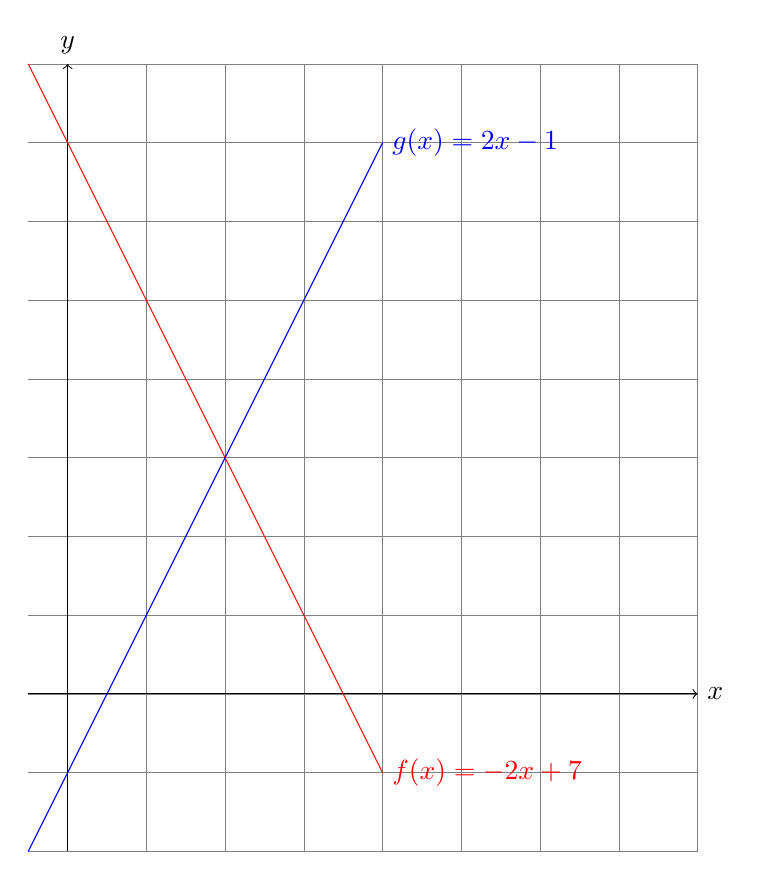
\begin{tikzpicture}
% tegn koordinatsystem
\draw[very thin,color=gray] (-0.5,-2) grid (8,8);
 \draw[->] (-0.5,0) -- (8,0) node[right] {$x$}; 
 \draw[->] (0,-2) -- (0,8) node[above] {$y$};
 % tegn linier
\draw[color=red][domain=-0.5:4]    plot (\x,-2* \x  + 7)             node[right] {$f(x) = -2x+7 $};
\draw[color=blue][domain=-0.5:4]    plot (\x,2* \x  - 1)             node[right] {$g(x) =2x-1$};
\end{tikzpicture}

\section*{Skæring mellem to 2. grads funktioner}
De to parabler: $$y = x^2 -4$$ og $$y = -x^2+4$$ skærer i
$$\begin{maxima}
  tex(solve(x^2-4=-x^2+4,x))
\end{maxima}$$

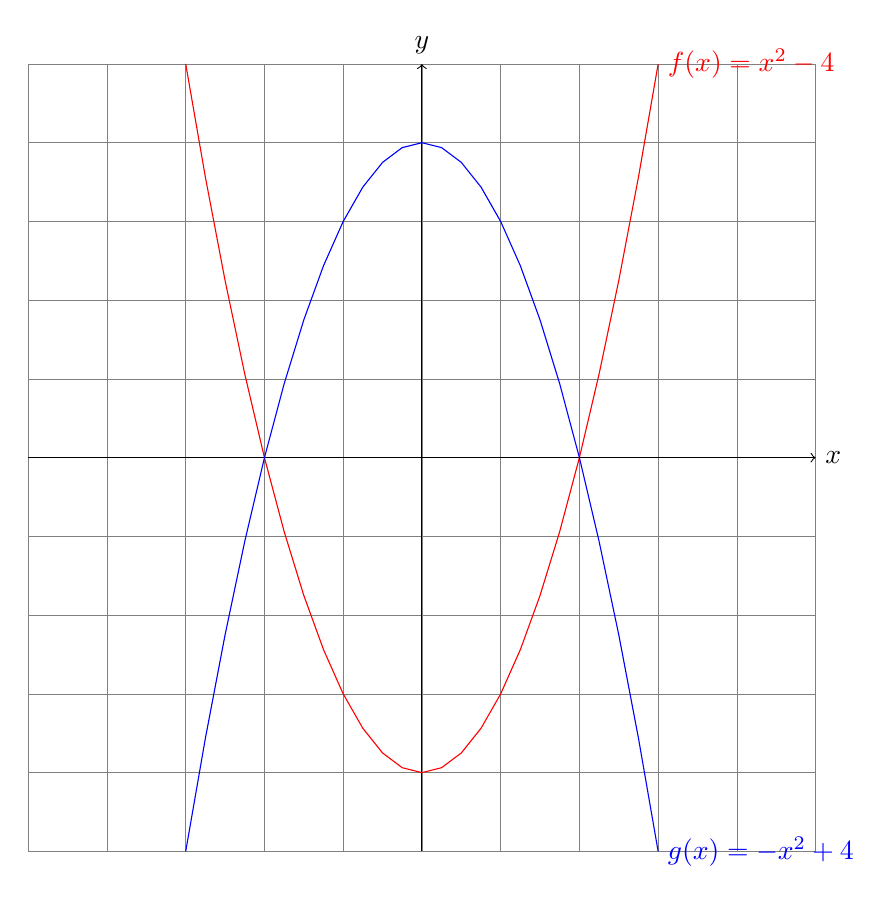
\begin{tikzpicture} 
% tegn koordinatsystem
 \draw[very thin,color=gray] (-5,-5) grid (5,5);
 \draw[->] (-5,0) -- (5,0) node[right] {$x$}; 
 \draw[->] (0,-5) -- (0,5) node[above] {$y$};
 % tegn linier
\draw[color=red][domain=-3:3]    plot (\x, \x*\x  - 4)             node[right] {$f(x) = x^2-4$};
\draw[color=blue][domain=-3:3]    plot (\x,-1 * \x * \x + 4 )             node[right] {$g(x) =-x^2+4$};
\end{tikzpicture}

\end{document}